\hypertarget{mtk__bc__descriptor__2d_8cc}{\section{src/mtk\+\_\+bc\+\_\+descriptor\+\_\+2d.cc File Reference}
\label{mtk__bc__descriptor__2d_8cc}\index{src/mtk\+\_\+bc\+\_\+descriptor\+\_\+2d.\+cc@{src/mtk\+\_\+bc\+\_\+descriptor\+\_\+2d.\+cc}}
}


Enforces boundary conditions in either the operator or the grid.  


{\ttfamily \#include \char`\"{}mtk\+\_\+tools.\+h\char`\"{}}\\*
{\ttfamily \#include \char`\"{}mtk\+\_\+bc\+\_\+descriptor\+\_\+2d.\+h\char`\"{}}\\*
Include dependency graph for mtk\+\_\+bc\+\_\+descriptor\+\_\+2d.\+cc\+:\nopagebreak
\begin{figure}[H]
\begin{center}
\leavevmode
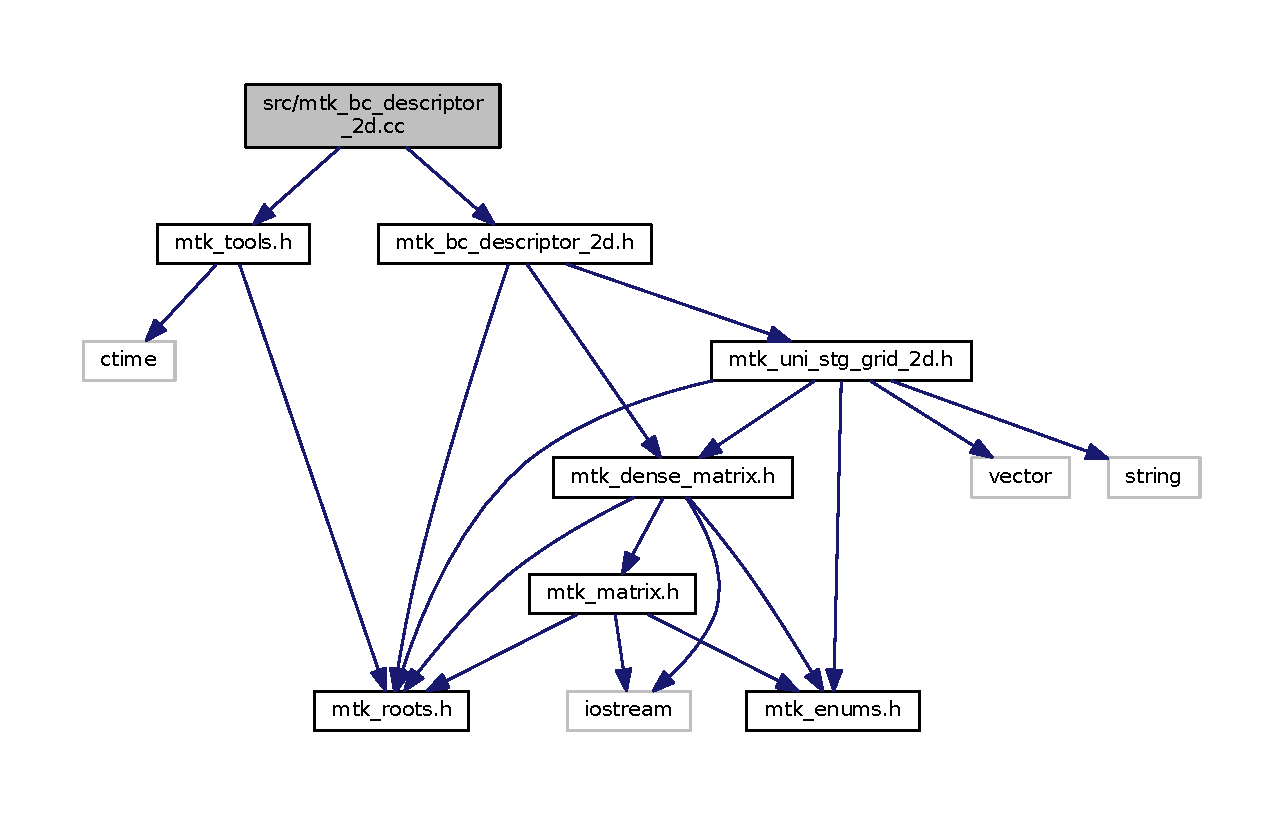
\includegraphics[width=350pt]{mtk__bc__descriptor__2d_8cc__incl}
\end{center}
\end{figure}


\subsection{Detailed Description}
This class presents an interface for the user to specify boundary conditions on 2\+D mimetic operators and the grids they are acting on.

{\bfseries Def.} Let $ f $ be any scalar or vector field defined over a domain $ \Omega $. We can specify any linear combination of $ f $ and its $ n $ derivatives to fulfill a condition, which we define as a {\bfseries boundary condition}\+:

\[ \forall \mathbf{x} \in \partial\Omega: \sum_{i = 0}^{n} c_i(\mathbf{x}) <\hat{\mathbf{n}}, \frac{\partial^i f}{\partial x^i}(\mathbf{x})> = \beta(\mathbf{x}). \]

This class receives information about the highest-\/order of differentiation, $ n $, all possible coefficient functions, $ c_i(\mathbf{x}) $ for any subset of the boundary (south, north, west and east), and each condition for any subset of the boundary, and takes care of assigning them to both, the differentiation matrices and the grids.

\begin{DoxyAuthor}{Author}
\+: Eduardo J. Sanchez (ejspeiro) -\/ esanchez at mail dot sdsu dot edu 
\end{DoxyAuthor}


Definition in file \hyperlink{mtk__bc__descriptor__2d_8cc_source}{mtk\+\_\+bc\+\_\+descriptor\+\_\+2d.\+cc}.

